\section{Λειτουργίες του Συστήματος}
Η αλληλεπίδραση του χρήστη με το συνολικό σύστημα γίνεται μέσω του ψηφιακού βοηθού. Όπως αναφέρθηκε στο \autoref{sec:rasa}, η κατανόηση των επιθυμιών του χρήστη και η ανίχνευση οντοτήτων είναι βασικά κομμάτια της επικοινωνίας χρήστη-συστήματος. Αρχικά, το σύστημα πρέπει να μπορεί να αναγνωρίζει γενικά \emph{intents} του χρήστη όπως χαιρετισμό/αποχαιρετισμό (\emph{greet/goodbye}), κατανόηση θετικής/αρνητικής απάντησης (\emph{affirm/deny}) και καλής/κακής διάθεσης (\emph{mood\_great/mood\_unhappy}). Οι λειτουργίες αυτές είναι βοηθητικές για την εξοικείωση του χρήστη με το σύστημα και έχουν εφαρμογή σε πολλών ειδών ψηφιακούς βοηθούς. Παράλληλα, υποστηρίζονται δύο ακόμη λειτουργίες μία για κατανόηση επιθυμίας του χρήστη για ερώτηση και μία για ανανέωση της βάσης σε πραγματικό χρόνο. Επιπλέον, υποστηρίζεται αναγνώριση της οντότητας του χρόνου, ώστε η αναζήτηση του χρήστη να γίνεται από συγκεκριμένο χρονικό διάστημα και έπειτα. Οι ενέργειες στις οποίες προβαίνει ο ψηφιακός βοηθός μπορεί να είναι μία απλή απάντηση (\emph{utter}, στατική χωρίς την εκτέλεση κάποιου κώδικα) ή δυναμική (\emph{action}, με εκτέλεση κώδικα στο παρασκήνιο) ή και τα δύο. 

Με βάση τα παραπάνω μπορούν να οριστούν οι βασικές λειτουργίες του συστήματος και η αντιστοίχηση των \emph{intents} του χρήστη με τις ενέργειες (\emph{utter/actions}) του ψηφιακού βοηθού ($\emph{intent} \rightarrow \emph{utter/action}$).
\begin{itemize}
    \item Χαιρετισμός/Αποχαιρετισμός του χρήστη \\
    $(\emph{greet/goodbye} \rightarrow \emph{utter\_greet/utter\_goodbye})$
    \item Κατανόηση της επιθυμίας του χρήστη για ερώτηση και αποστολή στο σύστημα που είναι στημένο στο \emph{Haystack} \\
    $(\emph{answer\_question} \rightarrow \emph{utter\_answer\_question} \rightarrow \emph{bot\_answer\_question})$
    \item Παρουσίαση της απάντησης που επέστρεψε το \emph{Haystack} μαζί με χρήσιμες πληροφορίες
    \item Υποστήριξη εντολών για την \emph{on-demand} ανανέωση της βάσης δεδομένων \\
    $(\emph{db\_update} \rightarrow \emph{utter\_db\_update} \rightarrow \emph{db\_update})$
\end{itemize}

\begin{figure}[!ht]
  \centering
  \captionsetup{justification=centering}
  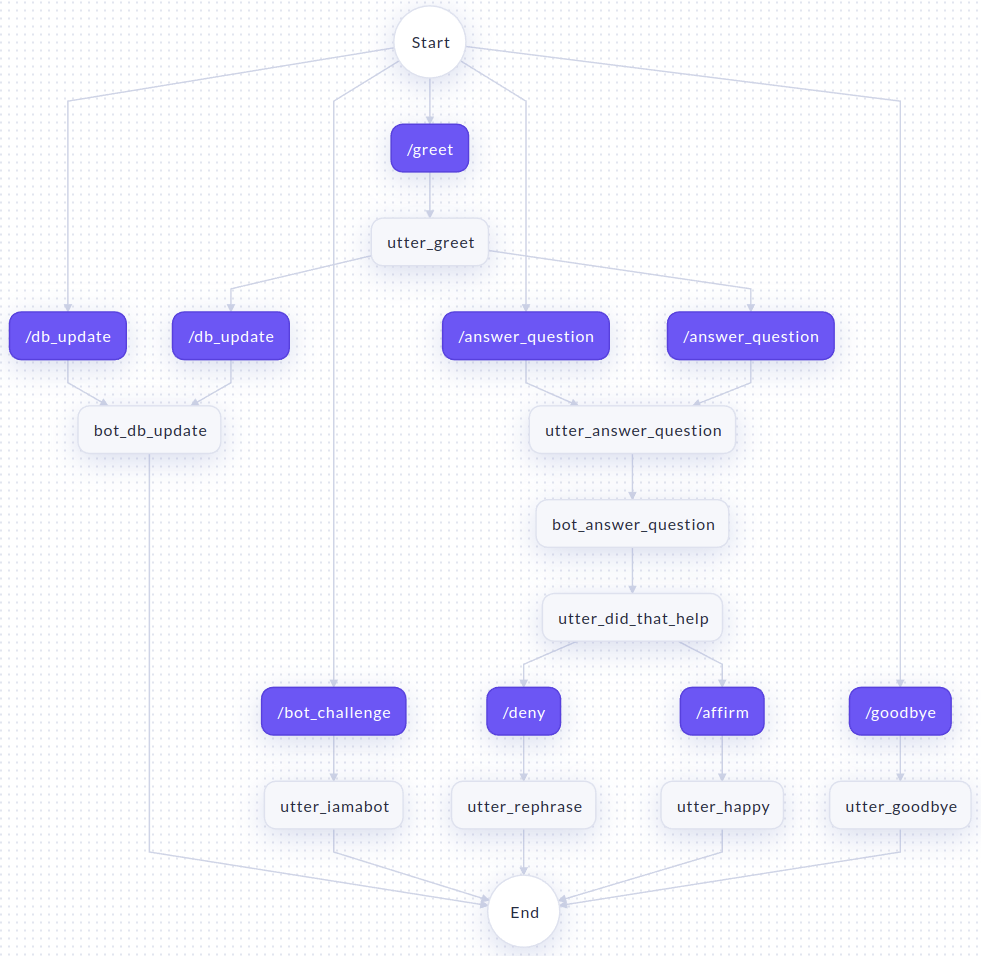
\includegraphics[width=1\textwidth]{images/chapter4/stories.png}
  \caption{Παράδειγμα ιστοριών στο περιβάλλον \emph{RASA-X}}
  \label{fig:stories}
\end{figure}
\noindent

Στο \autoref{fig:stories} παρουσιάζονται μερικά από τα μονοπάτια που μπορεί να ακολουθήσει η συζήτηση ψηφιακού βοηθού-χρήστη. Τα μονοπάτια αυτά ονομάζονται ιστορίες (\emph{stories}). Πιο συγκεκριμένα, ο βοηθός εκπαιδεύεται αρχικά με ένα σύνολο από \emph{stories} και στη συνέχεια μπορούν να προστεθούν ή να αφαιρεθούν ιστορίες, αναλόγως με την επιθυμητή συμπεριφορά.


Παράλληλα, στα σχήματα \ref{fig:example-1}, \ref{fig:example-2}, παρουσιάζονται δύο πραγματικές συνομιλίες με το σύστημα που αναπτύχθηκε. Ο βοηθός απαντάει σε κάθε ερώτηση του χρήστη παρέχοντας την απάντηση αλλά και το \emph{link} με την ιστοσελίδα από την οποία προήλθε, για περαιτέρω ανάγνωση της είδησης. Επιπλέον, ο χρήστης μπορεί να συνεχίζει την εισαγωγή ερωτήσεων στο σύστημα για όσο ο ίδιος επιθυμεί. Σε κάθε ερώτηση ο χρήστης ρωτάται αν η απάντηση ήταν αυτή που έψαχνε και σε περίπτωση που δεν ήταν τότε του ζητείται να αναδιατυπώσει την ερώτηση.

\begin{figure}[!ht]
\centering
\begin{minipage}{0.5\textwidth}
  \captionsetup{justification=centering}
  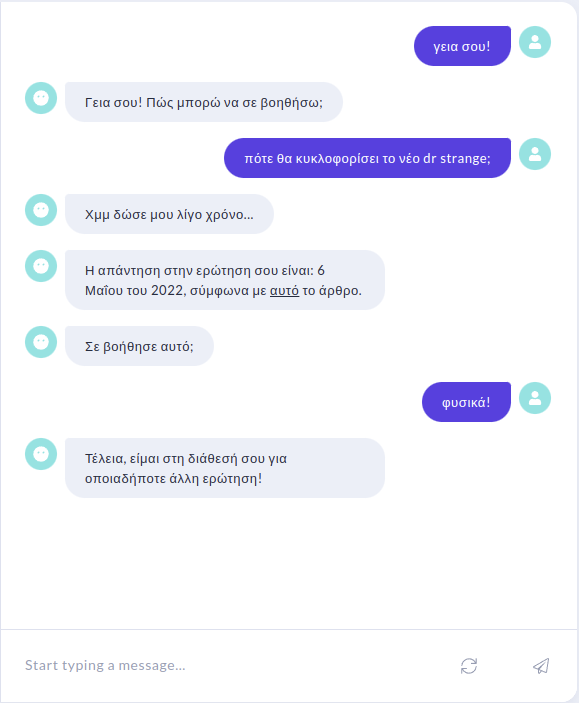
\includegraphics[width=1\textwidth]{images/chapter4/rasa-x-example-1.png}
\noindent
\caption{Παράδειγμα συζήτησης}
\label{fig:example-1}
\end{minipage}%
\begin{minipage}{0.5\textwidth}
  \captionsetup{justification=centering}
  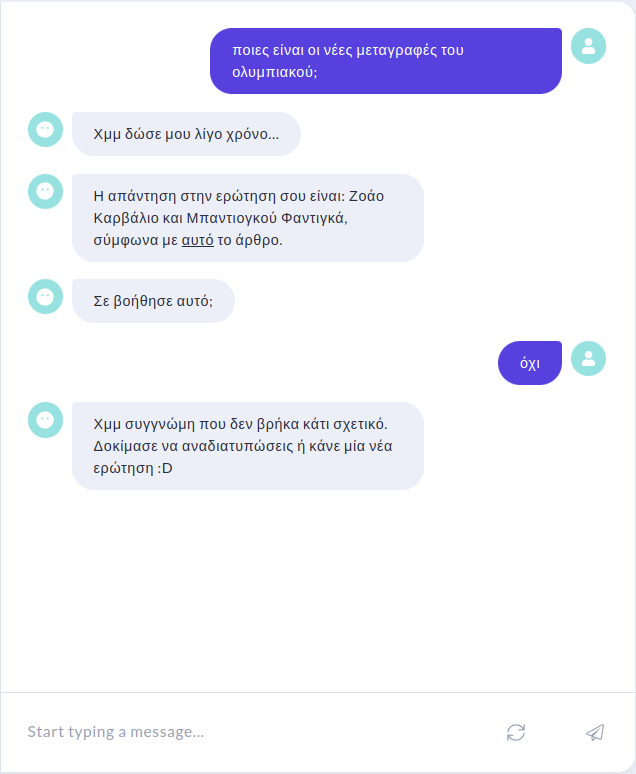
\includegraphics[width=1\textwidth]{images/chapter4/rasa-x-example-2.png}
\noindent
\caption{Παράδειγμα συζήτησης}
\label{fig:example-2}
\end{minipage}
\end{figure}

\section{Συνολικό σύστημα}
\label{sec:qasystem}
Η λειτουργία του συνολικού συστήματος μπορεί να παρουσιαστεί με το \linebreak \autoref{fig:qasystem}. Αρχικά, γίνεται η υπόθεση ότι υπάρχει ένα εξωτερικό σύστημα το οποίο παρέχει πρόσφατα άρθρα ειδήσεων. Τα άρθρα αυτά, καθώς φτάνουν στο σύστημα που αναπτύχθηκε, περνούν από έναν ταξινομητή ο οποίος ανιχνεύει τον τύπο του άρθρου (οι τύποι που υποστηρίζει ο ταξινομητής είναι πολιτικά, αθλητικά, τεχνολογία, ταινίες, \emph{gaming} και άλλο) και στην συνέχεια αποθηκεύονται στη βάση δεδομένων μαζί με τη πληροφορία της ταξινόμησης. Ως είσοδος του χρήστη στο σύστημα ορίζεται οτιδήποτε εισάγει με το πληκτρολόγιο στην επικοινωνία του με τον ψηφιακό βοηθό. Στη συνέχεια, το \emph{RASA} επεξεργάζεται την είσοδο του χρήστη και εξάγει την επιθυμία του. Αν ανιχνευτεί ότι ο χρήστης έκανε ερώτηση στο σύστημα τότε αυτή οδηγείται στο \emph{Haystack} το οποίο αναζητά την απάντηση στα άρθρα της βάσης δεδομένων και επιστρέφει την πιο πιθανή απάντηση.

\begin{figure}[!ht]
  \centering
  \captionsetup{justification=centering}
  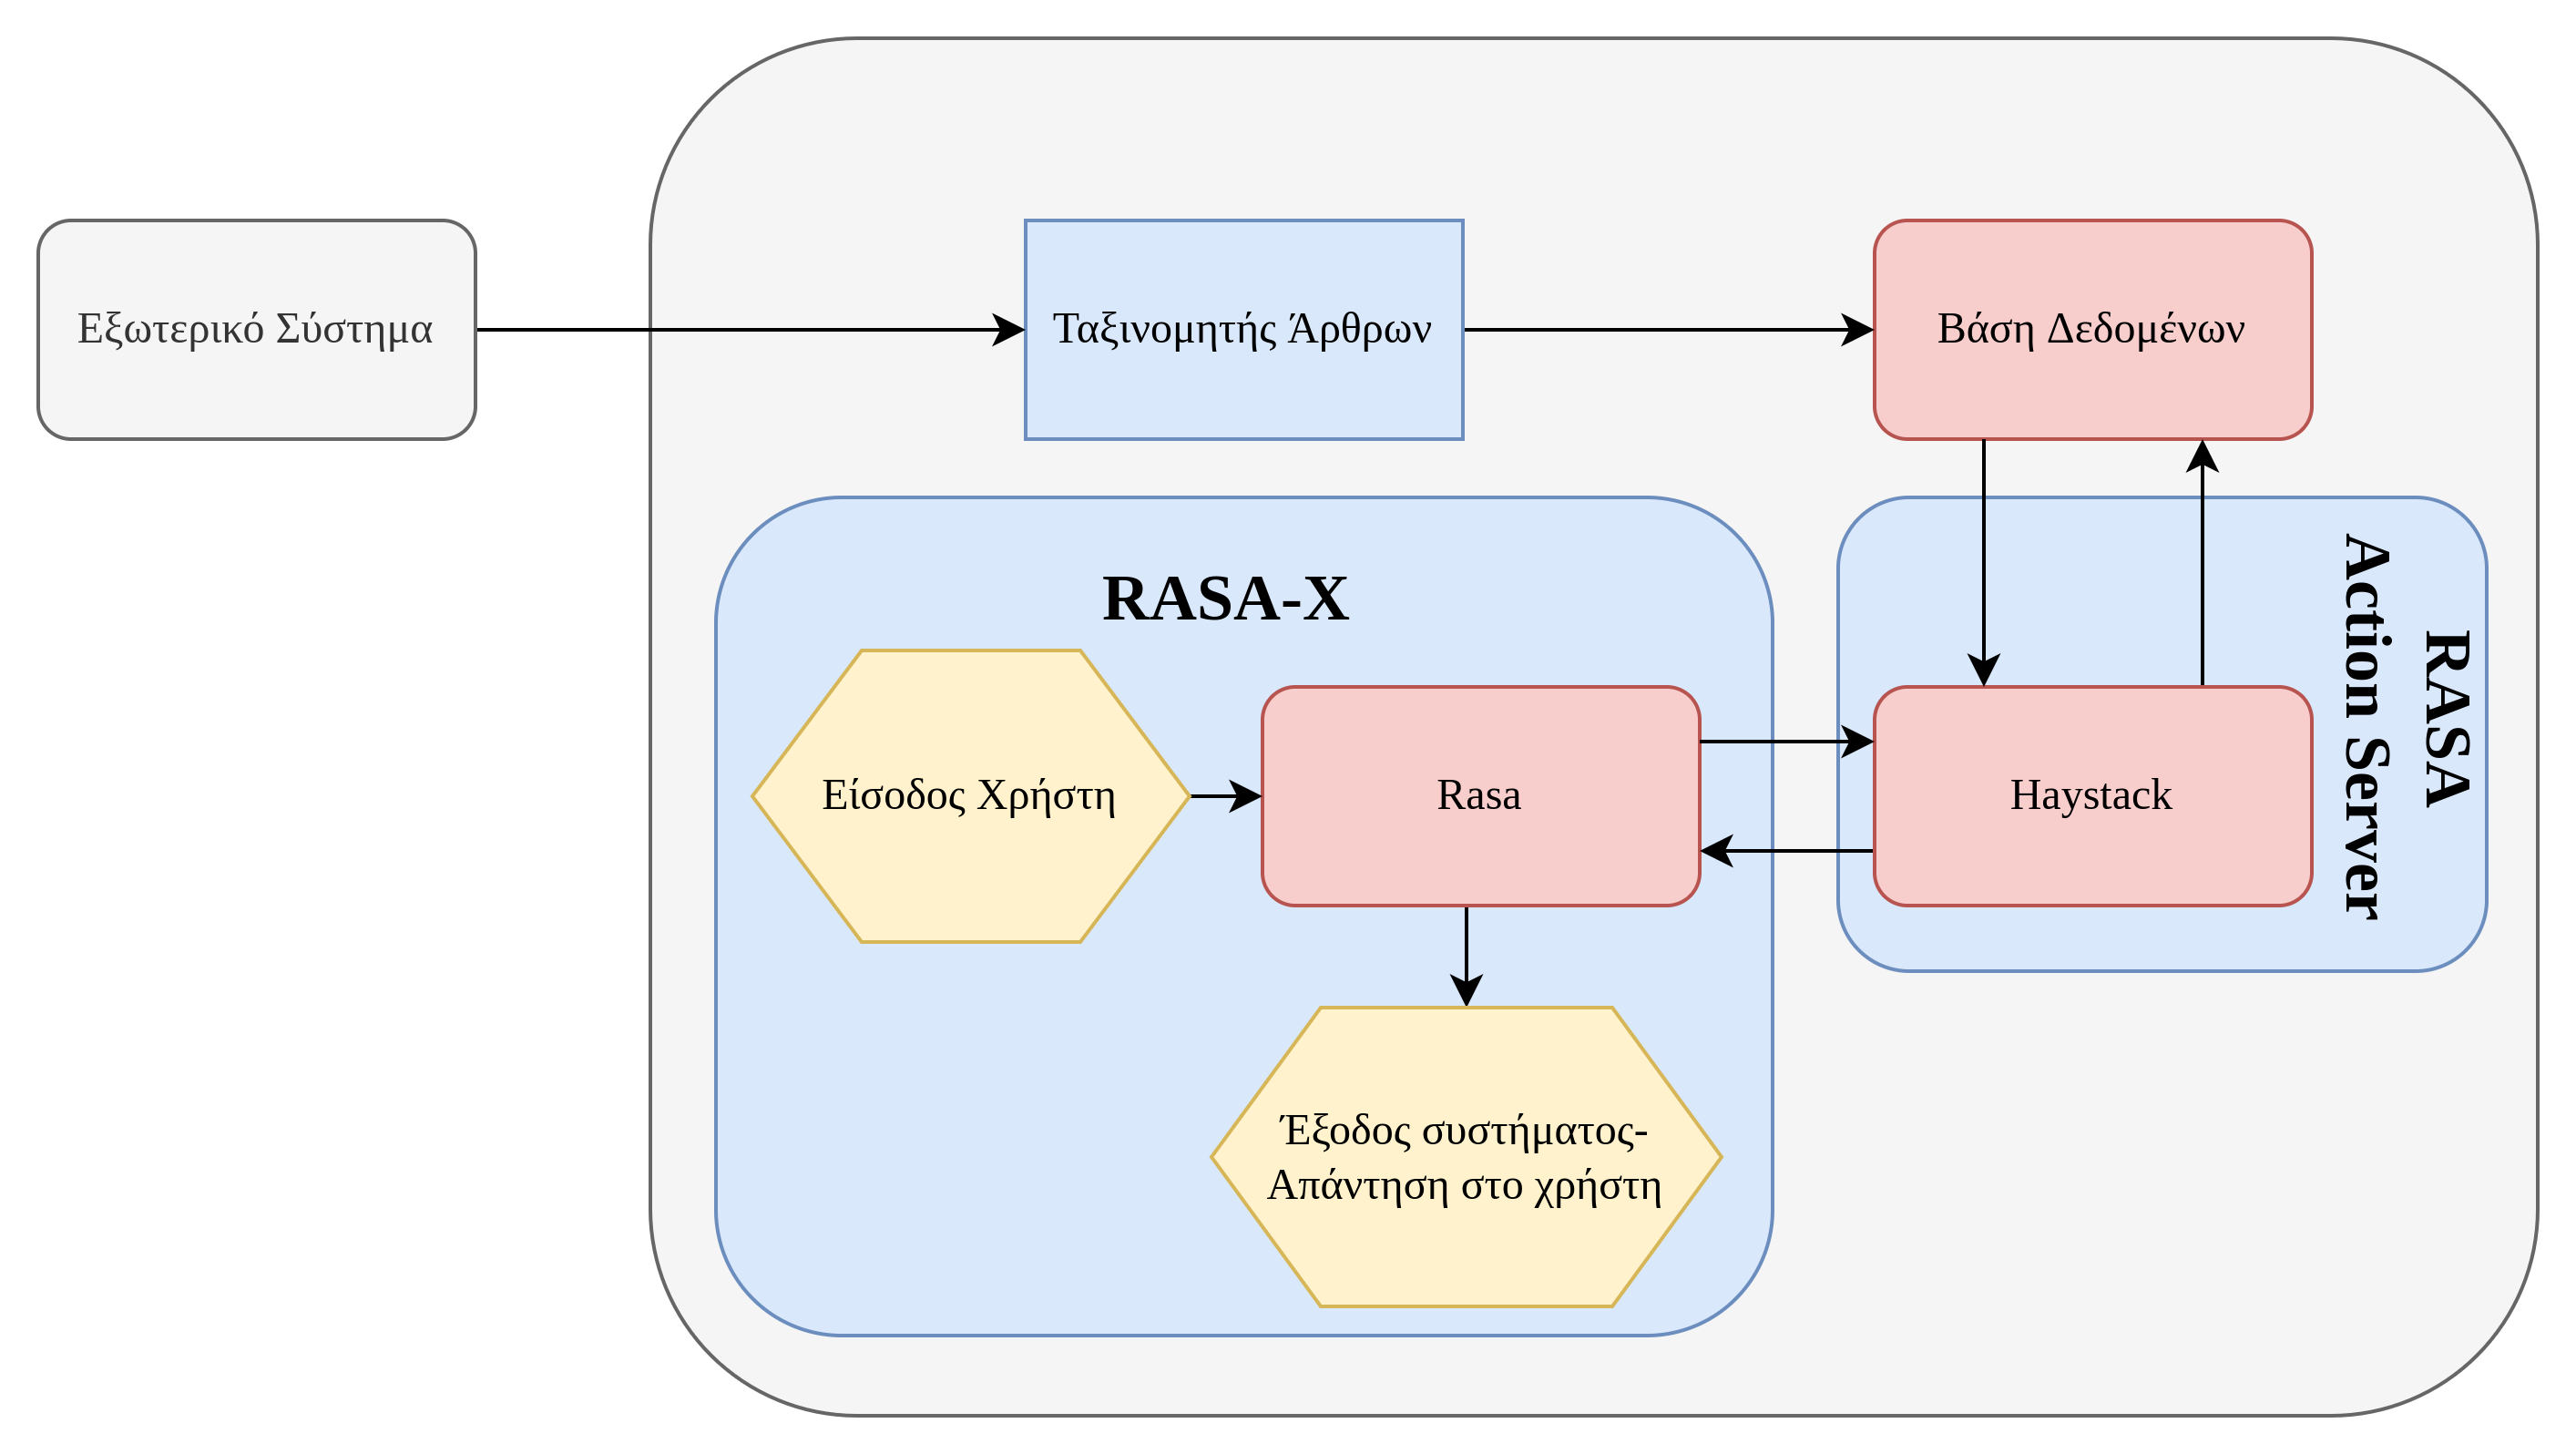
\includegraphics[width=1\textwidth]{images/chapter4/qasystem.png}
  \caption{Συνολικό σύστημα}
  \label{fig:qasystem}
\end{figure}
\noindent